\documentclass[a4paper]{article}

\usepackage{pgfplots}

\begin{document}

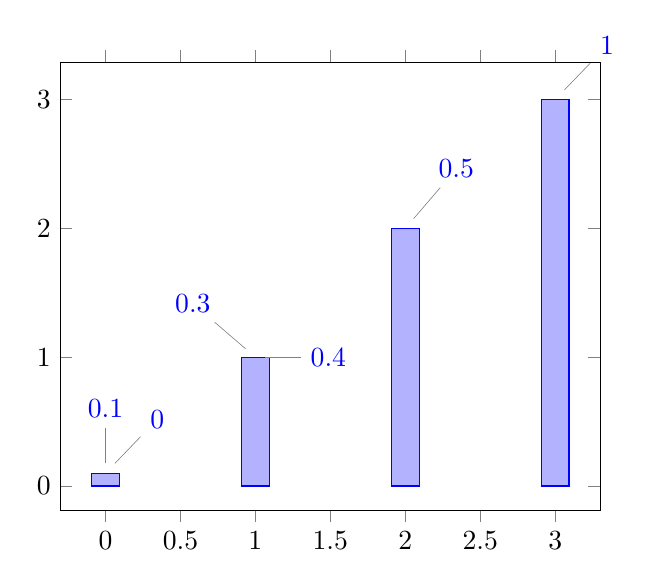
\begin{tikzpicture}
	\begin{axis}[clip=false,ybar]
	\addplot coordinates {(0,0.1) (1,1) (2,2) (3,3)} 
		node[pos=0,pin=45:0] {}
		node[pos=0.1,pin=90:0.1] {}
		node[pos=0.3,pin=135:0.3] {}
		node[pos=0.4,pin=0:0.4] {}
		node[pos=0.5,pin=60:0.5] {}
		node[pos=1,pin=45:1] {}
	;
	\end{axis}
\end{tikzpicture}

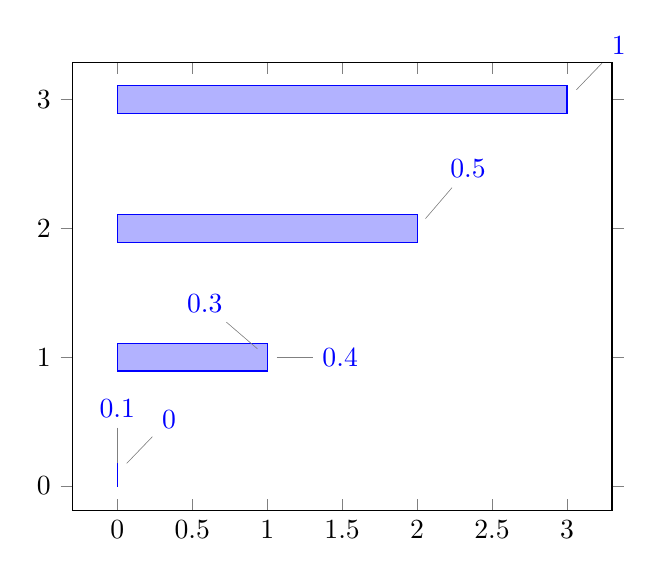
\begin{tikzpicture}
	\begin{axis}[clip=false,xbar]
	\addplot coordinates {(0,0.1) (1,1) (2,2) (3,3)} 
		node[pos=0,pin=45:0] {}
		node[pos=0.1,pin=90:0.1] {}
		node[pos=0.3,pin=135:0.3] {}
		node[pos=0.4,pin=0:0.4] {}
		node[pos=0.5,pin=60:0.5] {}
		node[pos=1,pin=45:1] {}
	;
	\end{axis}
\end{tikzpicture}
\end{document}

